\documentclass[crop=false, class=memoir]{standalone}
\usepackage[utf8]{inputenc}%Nødvendig for danske bogstaver
\usepackage[danish]{babel}%Sørger for at ting LaTeX gør automatisk er på dansk
\usepackage{csquotes}
\usepackage{geometry}%Til opsætning af siden
\geometry{lmargin = 2.5cm,rmargin = 2.5cm}%sætter begge magner
\usepackage{lipsum}%Fyldtekst, til brug under test af layoutet
\usepackage{float}
\usepackage{graphicx}%Tillader grafik
\usepackage{epstopdf}%Tillader eps filer
\usepackage{marginnote}% Noter i margen
\interfootnotelinepenalty=10000 %undgår at fodnoter bliver spilittet op.
\usepackage[sorting=none]{biblatex}
\addbibresource{litteratur.bib}
\usepackage[hidelinks]{hyperref}%Tillader links
\usepackage{subcaption} % Tillader underfigurer
\usepackage[font={small,sl}]{caption}	% Caption med skrå tekst ikke kursiv

\usepackage{xcolor} %Bruges til farver
\usepackage{forloop} %Bruges til nemmere for loops

\newcounter{opgave}[chapter] %Definerer opgavenumrene og hvornår de nulstilles
\renewcommand{\theopgave}{\thechapter.\arabic{opgave}} %Definerer udseende af opgavenummereringen
\newcounter{delopgave}[opgave] %Definerer delopgavenumrene
\newcounter{lvl} %Definerer en "variabel" til senere brug

\definecolor{markerColor}{rgb}{0.0745098039, 0.262745098, 0.584313725} %Definerer farven af markøren
\newcommand{\markerSymbol}{\ensuremath{\bullet}} %Definerer tegnet for markøren
\newlength{\markerLength} %Definerer en ny længde
\settowidth{\markerLength}{\markerSymbol} %Sætter den nye længde til bredden af markøren

\newenvironment{opgave}[2][0]{%Definerer det nye enviroment, hvor sværhedsgraden er den første parameter med en default på 0
\newcommand{\opg}{\refstepcounter{delopgave}\par\vspace{0.1cm}\noindent\textbf{\thedelopgave)\space}}%Definerer kommando til delopgave
\refstepcounter{opgave}%Forøger opgavenummer med 1 og gør den mulig at referere til
\setcounter{lvl}{#1}%Sætter "variablen" lvl lig med angivelsen af sværhedsgraden
\noindent\hspace*{-0.75em}\hspace*{-\value{lvl}\markerLength}\forloop{lvl}{0}{\value{lvl}<#1}{{\color{markerColor}\markerSymbol}}\hspace*{0.75em}%Sætter et antal af markører svarende til sværhedsgraden
\textbf{Opgave \theopgave : #2}\newline\nopagebreak\ignorespaces}{\bigskip} %Angiver udseende af titlen på opgaverne samt mellemrummet mellem opgaver



\usepackage{mathtools}%Værktøjer til at skrive ligninger
\renewcommand{\phi}{\varphi}%Vi bruger varphi
\renewcommand{\epsilon}{\varepsilon}%Vi bruger varepsilon
\usepackage{physics}%En samling matematikmakroer til brug i fysiske ligninger
\usepackage{braket}%Simplere kommandoer til bra-ket-notation
\usepackage{siunitx}%Pakke der håndterer SI enheder godt
\DeclareSIUnit\clight{\text{\ensuremath{c}}} % Lysets fart i vakuum som c og ikke c_0
\usepackage{chemmacros}
\usechemmodule{isotopes}
\usepackage{tikz}
\usepackage[danish]{cleveref}
\usepackage{nicefrac}
% \renewcommand{\ref}[1]{\cref{#1}}
\creflabelformat{equation}{#2(#1)#3}
\crefrangelabelformat{equation}{#3(#1)#4 to #5(#2)#6}
\crefname{equation}{ligning}{ligningerne}
\Crefname{equation}{Ligning}{Ligningerne}
\crefname{section}{afsnit}{afsnitene}
\Crefname{section}{Afsnit}{Afsnitene}
\crefname{figure}{figur}{figurene}
\Crefname{figure}{Figur}{Figurene}
\crefname{table}{tabel}{tabellerne}
\Crefname{table}{Tabel}{Tabellerne}
\crefname{opgave}{opgave}{opgaverne}
\Crefname{opgave}{Opgave}{Opgaverne}
\crefname{delopgave}{delopgave}{delopgaverne}
\Crefname{delopgave}{Delopgave}{Delopgaverne}

\newcommand{\eqbox}[1]{\begin{empheq}[box=\fbox]{align}
	\begin{split}
	#1
	\end{split}
\end{empheq}}

\newcommand{\kb}{\ensuremath{k_\textsc{b}}}

\DeclareSIUnit{\parsec}{pc}
\DeclareSIUnit{\lightyear}{ly}
\DeclareSIUnit{\astronomicalunit}{AU}
\DeclareSIUnit{\year}{yr}
\DeclareSIUnit{\solarmass}{M_\odot}
\DeclareSIUnit{\solarradius}{R_\odot}
\DeclareSIUnit{\solarluminosity}{L_\odot}
\DeclareSIUnit{\solartemperature}{T_\odot}
\DeclareSIUnit{\earthmass}{M_\oplus}
\DeclareSIUnit{\earthradius}{R_\oplus}
\DeclareSIUnit{\jupitermass}{M_J}

% Infobokse og lignende
% http://mirrors.dotsrc.org/ctan/graphics/awesomebox/awesomebox.pdf
% \usepackage{awesomebox}


% Egen infobokse (virker kun med begrænsede symboler)

\usepackage[framemethod=tikz]{mdframed}
\usetikzlibrary{calc}
\usepackage{kantlipsum}

\usepackage[tikz]{bclogo}

\tikzset{
    % lampsymbol/.style={scale=2,overlay}
    % lampsymbol/.pic={\centering\tikz[scale=5]\node[scale=10,rotate=30]{\bclampe}}.style={scale=2,overlay}
    infosymbol/.style={scale=2,overlay}
}

\newmdenv[
    hidealllines=true,
    nobreak,
    middlelinewidth=.8pt,
    backgroundcolor=blue!10,
    frametitlefont=\bfseries,
    leftmargin=.3cm, rightmargin=.3cm, innerleftmargin=2cm,
    roundcorner=5pt,
    % skipabove=\topsep,skipbelow=\topsep,
    singleextra={\path let \p1=(P), \p2=(O) in ($(\x2,0)+0.92*(1.1,\y1)$) node[infosymbol] {\bcinfo};},
    % singleextra={\path let \p1=(P), \p2=(O) in ($(\x2,0)+0.5*(2,\y1)$) node[infosymbol] {\bcinfo};},
]{info}

% Skal bruges som
% \begin{info}[frametitle={Titel}]
%     Tekst
% \end{info}
\usepackage{import}
\begin{document}
\section{Termodynamik}

\begin{opgave}{Idealgasloven}

\opg Hvad er volumen af $N=10^{23}$ luftmolekyler ved stuetemperatur (300K) og atmosfæretryk ($10^5Pa$)?

\opg Hvis man har en robust lukket beholder fyldt med luft, og man fordobler temperaturen af luften, hvad vil der så ske med trykket? (Fordoblet, halveret eller uændret?)

\opg Hvis man i stedet har en ballon, og sammepresser den til halvdeleden af dens størrelse langsomt, således at temperaturen af luften i ballonen er konstant, hvad vil da ske med trykket i ballonen? (Fordoblet, halveret eller uændret?)

\end{opgave}

\begin{opgave}{Termodynamikkens 1.lov}

\noindent
Forestil en lukket beholder med et mobilt stempel som på opgavefiguren. Beholderen er fyldt med 1 liter hydrogengas under atmosfærisk tryk.

\begin{figure}[H]
    \centering
    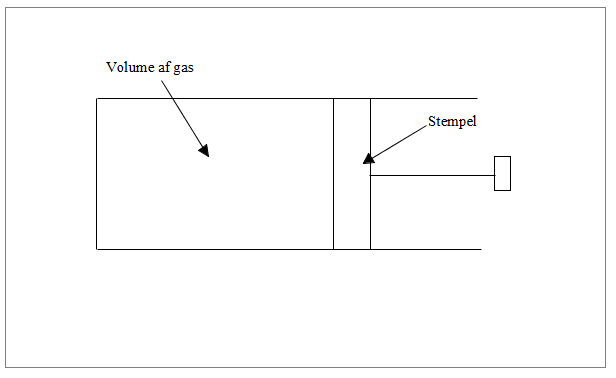
\includegraphics[scale=0.7]{Termodynamik/fig/Term1.png}
\end{figure}

\opg  Hvad er ændringen i den totale energi af gassen $\Delta U$, hvis stemplet er låst fast, og der tilføres 1kJ varme Q?

\noindent
Nu låses der op for stemplet, så den kan rykke sig.

\opg Hvis vi sammentrykker gassen så hurtigt, at der ingen varmeudveksling sker (adiabatisk process, hvor Q=0), og udfører et arbejde på 1kJ, hvad er så ændringen i den totale energi?

\opg Hvad den totale energi, hvis vi samtidigt sammentrykker gassen med et arbejde på 1kJ, og tilfører en varme på 1kJ?
\end{opgave}

\begin{opgave}{Mere 1. lov}

\noindent
Betragt den samme beholder som fra opg 1) fyldt med 1 liter hydrogengas ved stuetemperatur på \SI{20}{\celsius} og atmosfærisk tryk.

\opg Stemplet er låst fast igen, og temperaturen af hydrogengassen hæves fra \SI{20}{\celsius} til \SI{40}{\celsius}. Hvilken varme Q er blevet tilført beholderen?

\noindent
Beholderen er nu kølet ned til \SI{20}{\celsius} igen.

\opg Stemplet låses op nu. Stemplet sammentrykkes under konstant atmosfæretryk, sådan at gassens volumen formindskes til 0.5 liter. Hvilket arbejde er udført på gassen?

\opg Hvis ændringen i den totale energi er $\Delta U = 0$ for gassen efter sammentrykningen fra 2), hvad er så størrelsen af Q? Hvad er temperaturen af gassen? Forklar med din egne ord, hvad dette betyder. (Hurtig eller langsom sammentrykning?)

\opg Hvis ændringen i den totale energi i stedet er $W > \Delta U >0$ efter sammentrykningen, hvad er så fortegnet for Q? Er temperaturen mindre, større eller lig med \SI{20}{\celsius}? Hvad sker der denne gang? (Hurtig eller langsom sammentrykning?).

\opg Hvis ændringen for den totale energi er $\Delta U=W$, hvad er Q så efter sammentrykning? Hvad er størrelsen af temperaturen? Hvad sker der rent fysisk? (langsom, hurtig eller meget HURTIG sammentrykning?)

\end{opgave}

\begin{opgave}{Kredsprocess}

\noindent
Nedenfor ses et PV-diagram af en monoatomisk idealgas, der har 3 frihedsgrader.
\begin{figure}[H]
    \centering
    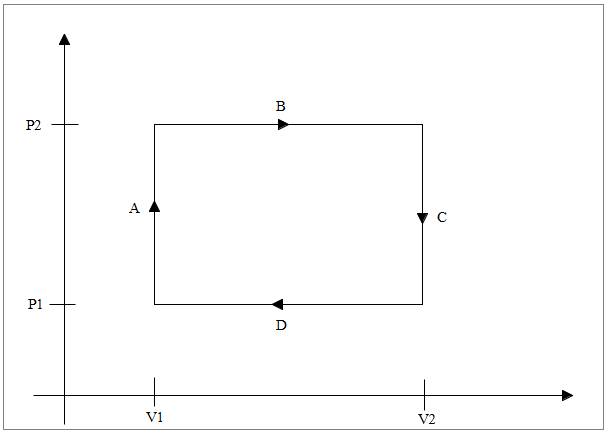
\includegraphics[scale=0.7]{Termodynamik/fig/Term3.png}
\end{figure}

\opg Afgør om arbejdet W er positiv, negativ eller 0 i de fire processer A-D.
\opg Afgør om ændringen i den totale energi $\Delta U$ er positiv, negativ eller 0 i de fire processer A-D.
\opg Afgør om varmetilførselen Q er positiv, negativ eller 0 i de fire processer A-D

\noindent
Det informeres, at $V1=1m^3$, $V2=2m^3$, $P1=1bar$ og $P2=2bar$

\opg Beregn W for de fire processer A-D
\opg Beregn $\Delta U$ for de fire processer A-D
\opg Beregn Q for de fire processer A-D
\opg Hvad er summen af W, summen af $\Delta U$ og summen af Q for de fire processer?

\noindent
Læg mærke til om et af summene svarer til arealet af figuren i PV-diagrammet.
\end{opgave}

\begin{opgave}{Kredsproccess2}

\noindent
Nedenfor ses et PV-diagram af $N=10^{25}$ dinitrogen gas, der har 5 frihedsgrader.

\begin{figure}[H]
    \centering
    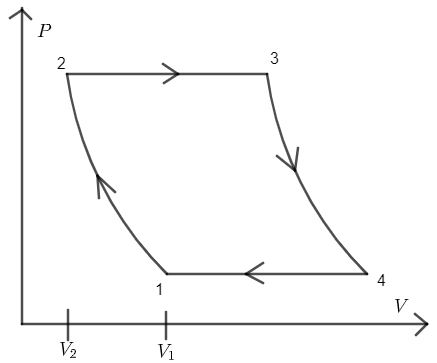
\includegraphics[scale=0.8]{Termodynamik/fig/Term4.png}
\end{figure}

\noindent
Kredsprocessen består af 4 processer:

\begin{itemize}
    \item Fra 1 $\longrightarrow$ 2 er en adiabatisk kompression
    \item Fra 2 $\longrightarrow$ 3 er en isobar ekspansion (Hvor gassen tilføres varme)
    \item Fra 3 $\longrightarrow$ 4 er en adiabatisk ekspansion
    \item Fra 4 $\longrightarrow$ 1 er en isboar kompression (Hvor gassen afgiver varme)
\end{itemize}

\noindent
Det vides, at $V_1=2m^3$, $V_2=1m^3$ og at $T_1=300K$

\opg Hvad er trykket i tilstand 1?
\opg Hvad er temperaturen i tilstand 2?
\opg Hvad er den totale energi af dinitrogen gassen i tilstand 2? \\

\noindent 
Det oplyses, at $V_3=3m^3$ \\

\opg Hvad er temperaturen i tilstand 3?
\opg Hvad er trykket i tilstand 3? \\

\noindent
Det oplyses nu, at $V_4=6m^3$ \\

\opg Hvad er temperaturen af tilstand 4?
\opg Bestem trykket af tilstand 4 (og dermed også af tilstand 1)  vha. den adibatiske formel for tryk og volumen. Er den det samme som trykket fundet i 1)?

\opg Bestem arbejdet fra 2 $\longrightarrow$ 3 og fra 4 $\longrightarrow$ 1.  
\opg Bestem arbejdet fra 1 $\longrightarrow$ 2 og fra 3 $\longrightarrow$ 4. (Husk at Q=0 for adiabatiske processer).
\opg Hvad er summen af arbejdet? Wow, hold da op! Du har lige bestemt arealet af figuren på en sej fysiker måde!

\end{opgave}

\begin{opgave}{Varmekapacitet udledningsopgave}

\noindent
Varmekapaciteten C er en størrelse, der fortæller en om, hvor meget varme skal man tilføre et system for at opvarme den 1 temperatur grad. Den er derfor givet ved:

\begin{equation*}
    C=\frac{Q}{\Delta T}
\end{equation*}

\noindent
Hvor Q er varmen tilført, og $\Delta T$ er temperatur ændringen grundet varmetilførslen. \\

\opg Brug termodynamikkens første lov til at udtrykke Q, og indsæt i ligningen ovenover.
\opg Forestil dig, at vi har at gøre med en ideal gas under konstant tryk. Anvend dette til at komme frem til, at $C=(\frac{\partial U}{\partial T})+P(\frac{\partial V}{\partial T}), \, P=konstant$. Hint: (Et smart fysiker trick er, at hvis du eksempelvis har $\frac{\Delta y}{\Delta x}=xz$, og hvis du gør $\Delta x$ og $\Delta y$ uendelige små, så bliver ligningen til $\frac{\partial y}{\partial x}=xz$!

\opg Anvend til sidst equipartitions teormet og idealgasligningen til at komme frem til, at $C=\frac{f}{2}Nk+Nk, for P=konstant$ \\

\noindent
(Man kan altså bestemme varmekapaciteten af en ideal gas under eksempelvis konstant atmosfæretryk, så længe man kender f og N af gassen. Ej hvor sejt!)

\end{opgave}

\begin{opgave}{Lille entropi opgave}

\noindent
I denne opgave vil vi prøve at give en god ide om, hvordan entropi fungerer. Betragt et hydrogen atom, der har en elektron og to tilstande som elektronen kan være i. En figur nedenfor illustrerer dette.

\begin{figure}
    \centering
    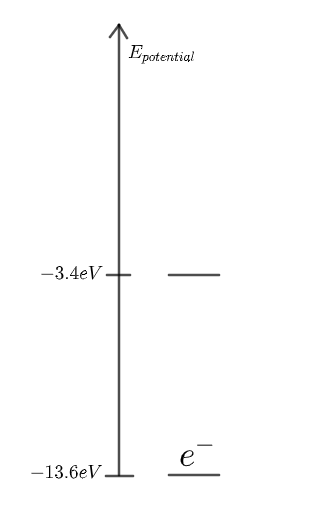
\includegraphics[scale=0.4]{Termodynamik/fig/Termentro.png}
\end{figure}

\noindent
Elektronen kan altså være i to forskellige tilstande, og da er multipliciteten af hydrogenatomet 2. Forestil nu, at vi betragter et magen til hydrogenatom, der er på vej hen mod vores hydrogen atom for at reagere med det og danne H_{2}.

\opg Hvis vores system er disse to hydrogenatomer, hvad er så den samlede entropi af systemet, inden de støder sammen?

\noindent
Nu reagerer de spontant sammen og danner $H_{2}$, og da bliver systemet til:

\begin{figure}
    \centering
    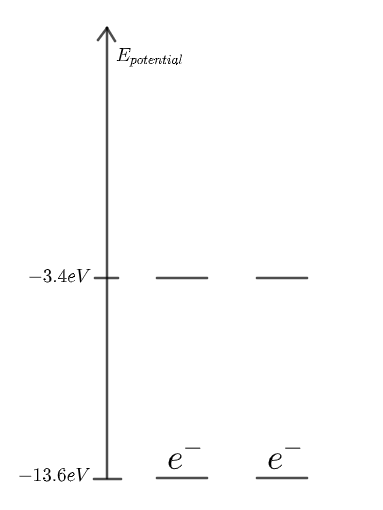
\includegraphics[scale=0.4]{Termodynamik/fig/Termoentro2.png}
\end{figure}

\opg Hvad er multipliciteten af $H_{2}?$ Altså på hvor mange forskellige måde kan du fordele elektronerne? (Husk at man ikke kan se forskel på elektronerne)
\opg Hvad er den samlede entropi af systemet nu? Er den større eller mindre end i 1)? \\

\noindent
Der ser man bare. Entropien er altså steget helt spontant i vores system uden nogen ydre påvirkninger! Dette viser sig at være gældende for alle lukkede systemer (selv universet).
\end{opgave}

\end{document}